\chapter{Reinforcement Learning Model}
\label{chap:RL}
\section{Introduction}
In the last session we analyzed the task-related activity patterns of principal assembly-pair types.\\Significant task related activity was tested with Friedman test in stimulus presentation (CS+/-) interval, stimulus continued\footnote{The window right before the reward delivery time, or the expected reward time in False Alarm trials, or the hypothetical reward time in Correct Rejection trials.} (CS+/- cont.) interval, and reward\footnote{Or expected reward in False Alarm trials, or Hypothetical Reward in Correct Rejection trials.}.\\We found a good portion of SPN-DAN pairs becoming active early at stimulus presentation, another important group being active later during the stimulus presentation, and only a small fraction of SPN-DAN pairs active only at the retrieval.\\The described activity pattern makes SPN-DAN pairs good candidates for reward prediction (RP) coding.\\On the other hand we observed that FSN-DAN pairs are early activated by the stimulus on onset and they show as well a phasic activity at the reward time.\\This kind of activity pattern suggests that FSN-DAN pairs could code for reward prediction error (RPE).\\However we are not able to address those question with the presented activity patterns description, that is rather static, whereas the performed task was highly dynamic.\\The task was such that the animal had to assign and re-assign a value to the rewarded odor to be able to predict the reward.\\To take into account the learning dynamic, we used the reinforcement learning technique \cite{SuttonBarto}. $"$Reinforcement learning$"$ is an area in machine learning, in which an agent tries to learn the best action to take, depending on the circumstances in which this action will be performed, this approach can incorporate any changes in the environment of the decision making process. In psychology, from where the idea of this machinery derives, the concept is known as “learning by reinforcement”: the agent receives a reward or punishment, depending on the decision made, through the experience he is able to associate the actions that generate the greatest reward for each situation that the environment presents, and to avoid unrewarded actions or actions that generate punishment.\\
Machine learning uses the same idea: the machine observes a state and, based on this, chooses an action to take and receives the reward associated with that specific action in that state, thus obtaining the information of this specific combination. The process is repeated until the machine is able to choose the best action to take for each of the possible scenarios to be observed in the future.\\In the contingencies of the experiment conducted in our lab, two odor were presented and only one was associated with a reward with a probability of 0.9. Each time one odor was presented the mouse chose to take the action (lick or not lick) that maximized the reward and minimized his effort. the task was learnt when the animal was able to lick for the rewarded odor and not lick when the unrewarded odor was presented.\\To model this learning process we set up a Rescorla Wagner model with Pearce Hall update mechanism (\cite{Li}, \cite{Costa}, \cite{Koppe}).\\

%%
%We use here Reinforcement Learning/Forgetting models (\cite{SuttonBarto}) with Q-learning values (\cite{Dayan1}) to fit mice behaviour in go-no go odor discrimination task; we regress afterwards neuronal activity with model values.
\section{Model}
%%%%%{\color{blue}Start writing equation of reinforcement learning}
%%%%%First Option I tried, Georgia's option {\color{red}cite Georgia's paper}
%%%%%We set up four RL models and we chose the one that better fitted the behaviour for the regression analysis.
Reinforcement learning model are usually set up as follows:
\begin{itemize}
    \item At each trial $t$ of the experiment, a state $s$ is observed, this is an input of the model.
    \item After the stimulus presentation, the animal has the chance to take an action, and according to choice made, the reward is delivered. The reward is a vector $r(t)$, each vector component indicates the reward value delivered at the trial $t$, the reward vector is an input of the model.
    \item After the reward delivery, the animal computes the reward prediction error, that is evaluated in the model as the difference between the actual reward and the expected reward.
    \item States values are the expected reward values and they are updated according to the last expected values and the reward prediction error and it is modulated by the learning rate.
    \item The learning rate is often a constant free parameter, however it has been shown that a time dependent variable better describes the learning dynamic (\cite{Funamizu},\cite{Daw}).
    \item Learned values are then translated into action probabilities via a softmax function, maximized with respect some free parameters.
\end{itemize}
We set up an hybrid Rescorla-Wagner/Pearce-Hall update mechanism following the scheme above
The V values are updated according to the equation
\begin{equation}
V_s(t+1)=V_s(t)+k\cdot\alpha_t\cdot\delta  \hspace{0.3cm} with \hspace{0.3cm}\delta(t)=r(t)-V_s(t)
\label{VValues}
\end{equation}

%%%%%%NOn da buttare
We set up a Q Learning-Forgetting model (Q L-F model) starting from an hybrid Rescorla-Wagner/Pearce-Hall update mechanism (\cite{Koppe}, \cite{Costa}, \cite{Li}) with update of unchosen option (\cite{Katahira}) and the associability related to the chosen and unchosen options, using learning and forgetting parameters ({\color{red} cite Dayan, literature on Q L-F models}).
The model assigns each state $s$ and action $a$, an action value $Q_{s,a}(t)$ where $t$ is the index of the trial. In our specific case we have two states, corresponding to the two odors presented and two possible actions, i.e., to lick or not to lick. 
Based on the set of action values the model transforms the The action value for the chosen option is updated by
\begin{equation}
Q_{s,a}(t+1)  = Q_{s,a}(t)+k_L\cdot\alpha_L(t)\cdot\delta(t), \hspace{0.3cm} with \hspace{0.3cm}\delta(t)=r(t)-Q_{s,a}(t)
\label{eq:Qlearning}
\end{equation}
where $\delta$ is the prediction error, i.e., the difference between the reward $r(t)$ and the expected reward value $Q_{s,a}(t)$ for an action $a$ given a state $s$, $k_L$ is the learning parameter and $\alpha_L(t)$ is the Pearce-Hall associability for the chosen option, is a trial-dependent rate component which adjusts in accordance with the average accuracy of recent predictions, evolving by
\begin{equation}
   \alpha_L(t)=(1-\eta)\cdot\alpha_L(t-1)+\eta\cdot\abs{\delta(t)},\hspace{0.3cm} \eta\in[0,1]
    \label{eq:Alphalearning}
\end{equation}
Note that the $n$'s associability depends on absolute prediction errors from past trials, but not the current one ensuring that $\delta(t)$ was not double counted in the value update. 
For the unchosen option $a'\neq a$ the action value is updated by
\begin{equation}
    Q_{s,a'}(t+1) = Q_{s,a'}(t)-k_F\cdot\alpha_F(t)\cdot Q_{s,a'}(t)
    \label{eq:Qforgetting}
\end{equation}
where $k_F$ is the forgetting rate (\cite{ItoDoya}) and the associability for the unchosen option is time-dependent and evolves as follows
\begin{equation}
    \alpha_F(t)=(1-\eta)\cdot\alpha_F(t-1)+\eta\cdot Q_{s,a'}(t-1), \hspace{0.3cm}
    \eta\in[0,1]
    \label{eq:Alphaforgetting}
\end{equation}
Note that using $k_F = 0$ the model is reduced to the basic Rescorla Wagner/Pearce Hall model. We applied to our data four different version of the model, the one shown here as presentation is the one that better fit the behavioural data. The other three versions are:
\begin{description}
    \item[i.] The presented model is reducible to an hybrid Rescorla Wagner/Pearce Hall update mechanism when we use a learning parameter $k$, and no forgetting parameter, i.e. $k_F = 0$.
    Then, if $a$ represents the chosen option and $a'\neq a$ the unchosen option, the action values evolve as follows\\
    $\begin{array}{lcl}
    Q_{s,a}(t+1)&=& Q_{s,a}(t)+k\cdot\alpha_L(t)\cdot\delta(t), \hspace{0.3cm} with \hspace{0.3cm}\delta(t)=r(t)-q_{s,a}(t)\\
    Q_{s,a'}(t+1)&=&Q_{s,a'}(t)\\
    \end{array}$
    \item[ii.] Let $a(t) \in \{1,0\}$ denote the option was chosen at trial $t$, where $1$ stands for "to lick" and $0$ stands for "not to lick". We introduce then two learning parameters $k_{1}$ and $k_{0}$ respectively for the choice $a=1$ and $a=0$ to be estimated by the model, while $k_F$ is fixed to zero.
    Then when the choice $a=1$ is realized, the action values evolves by\\
   $\begin{array}{lcl}
       Q_{s,1}(t+1)&=&Q_{s,1}(t)+k_1\cdot\alpha(t)\cdot\delta(t)\\
         Q_{s,0}(t+1)&=&Q_{s,0}(t)\\ 
    \end{array}$\\
    while if the choice $a=0$ is realized we have\\
    $\begin{array}{lcl}
       Q_{s,0}(t+1)&=&Q_{s,0}(t)+k_0\cdot\alpha(t)\cdot\delta(t)\\
         Q_{s,1}(t+1)&=&Q_{s,1}(t)\\ 
    \end{array}$
    \item[iii.] We use a learning model, without forgetting parameters, and we introduce two $\eta$ parameters $\eta_1$ and $\eta_0$ for the choice $1$ and $0$ respectively, to be estimated by model, in order to define two associability $\alpha_{L1}$ and $\alpha_{L0}$ evolving as follows:
   $\begin{array}{lcl}
    \alpha_{L1}(t) & = & (1-\eta_1)\cdot\alpha_{L1}(t-1)+\eta_1\cdot\abs{\delta(t)} \\
    \alpha_{L0}(t) & = & (1-\eta_0)\cdot\alpha_{L0}(t-1)+\eta_0\cdot\abs{\delta(t)} \\
    \end{array}$\\
    and action values for the chosen option evolving consequently as in the equation \ref{eq:Qlearning}.
\end{description}
\section{Behaviour Fit}
\label{sec:Behavior}
We compare the models and it resulted the Forgetting$-$Learning Model showing the best behavioural fit. We computed the mice performance and compared it with the action values, furthermore we used the Bayesian Information Criterion to establish which was the best model.\\

\begin{figure}[ht!]
    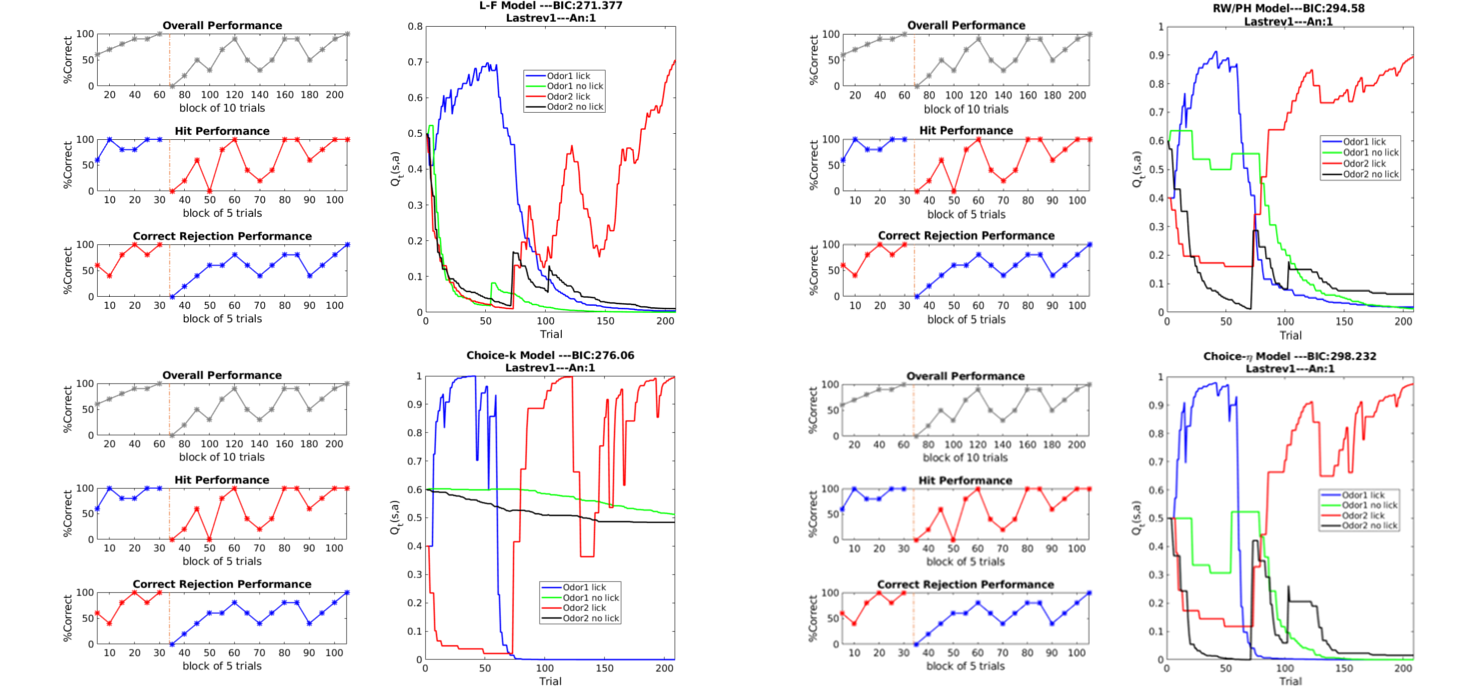
\includegraphics[scale=0.3]{figures/ResumeRLPerf.png}
    \caption{{\color{red} to be modified as follows: only one performance plot and plot comparison} In figure one example of animal performance and RL model action values.
    Odor 1 was rewarded only in the original phase, while Odor 2 was rewarded only in the reversal phase. Top: Performance in all trials, in hit trials and correct rejection trials. Bottom: RL model action values for the action lick, when odor 1/odor 2 occurs (blue/red) and the action no lick when odor 1/odor 2 is presented (green/black). Action values associated to lick for non rewarded odor and non-lick for rewarded odor give us an estimation of "false alarm" and "miss"trials, namely respectively trials in which the odor was not rewarded and the mouse went for the reward, or in which the odor was rewarded and the mouse sat quiet. Those trials at the beginning of the phase some trials.
    }
    \label{fig:PerfRL}
\end{figure}
In figure one example of animal performance and RL-models action values. When the odor is rewarded the expectancy of reward related to the lick action reproduce the hit performance as one could intuitively predict, while, for non rewarded odor, the reward expectation associated to the no-lick action decrease as the correct rejection performance increase. Action values associated to lick for non rewarded odor and non-lick for rewarded odor give us an estimation of $"$false alarm$"$ and $"$miss trials$"$, namely respectively trials in which the odor was not rewarded and the mouse went for the reward, or in which the odor was rewarded and the mouse sat quiet. That happened especially as the experiment or the new phase began for the first 5-10 trials of the phase.\\
From the Bayesian Information Criterion (BIC) the L-F model results to be the best model fig.(\ref{fig:BIC}), confirming the evidences of the action values plots in fig.(\ref{fig:PerfRL}).
\begin{figure}
    \centering
    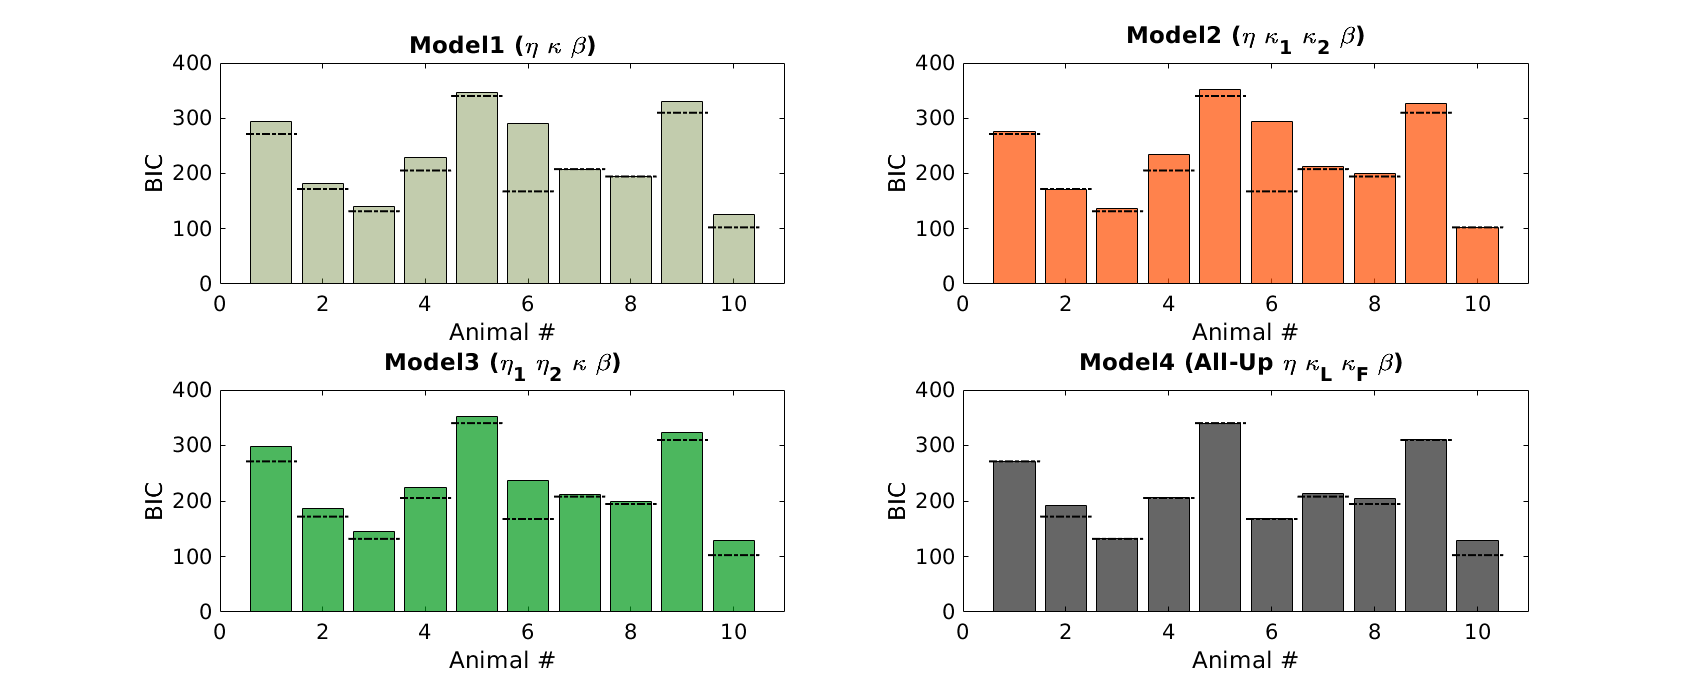
\includegraphics[scale=0.3]{figures/BIC_ModelCompare.png}
    \caption{{\color{red}Change figure and title of the plots} BIC Information Criterion for the four models implemented}
    \label{fig:BIC}
\end{figure}
To see whether the neural activity is correlated with the behaviour, we regress the neuronal activity and the assembly activity with the Q L-F model action values $Qs$, error prediction $\delta$, and associability $\alpha$ and behavioural measures. 
    
\section{Uncertainty and prediction error signal in pair-types}
\label{sec:CorrRL}
We carried out a multiple regression analysis of neuronal and assembly's activity by the four action values of the Q F-L model, $\delta(t)$, $\alpha_L(t)$ and $\alpha_F(t)$. To further test whether the neuronal and assembly activities were correlated with the parameters of subsequent lick movements, or the odor identity, we analyzed the residual components, $\epsilon(t)$, using lick related variables and the odor identity, namely, the mouse's action choice $a(t)$, the lick frequency within the lick-window $l_{in}(t)$, the lick frequency outside the lick-window, before the opening,$l_{out}(t)$ and the odor identity $o(t)$.
Thus we model the neuronal or assembly activity $y(t)$ during the post-stimulus, pre-reward and post-reward periods in the $t-th$ trial as follows:\\
\begin{equation}
\begin{cases}
y(t)=b_0+\sum\limits_{l}^{L} b_l\cdot M_l+\epsilon(t)\\
\epsilon(t)=\sum\limits_i^I c_i\cdot N_i
\end{cases}
\label{eq:MultiLinRe}
\end{equation}
where $y$ are the observations, the neuronal{\color{blue}/assembly's} activity in this case, $M$ is the ($T\times L$) regressor's Matrix of the Q L-F model part, where $T$ is the number of trials and $L$ the number of regressors. $M$ has as columns
the regressors of the model's part, namely, the vectors $Q_{1,1}$, $Q_{1,0}$, $Q_{2,1}$, $Q_{2,0}$, $\delta$, $\alpha_L$, $\alpha_F$; the set of values $b_m$ are regressor parameters or weights related to the model's regressors. $N$ is the ($T\times I$) regressor matrix of the residual part, where $I$ is the number of regressors of the residual part. N has as columns the regressors $a$, $l_{in}$, $l_{out}$ and $o$, while $c_i$ are the weights of the residual part.
Linear regression models assume response variables to be normally distributed. Neuronal responses are Poisson distributed (although the normal distribution is in this case a good approximation), {\color{blue} and assemblies show Gamma distribution,} thus considering our data distributions, we built a generalized linear model (GLM), with GLM is possible to generalize the simple linear regression by allowing for response variables that have arbitrary distributions and for an arbitrary function of response variables, the link function, to vary linearly with the predicted values, rather than assuming that the response itself must vary linearly. The mean $\mu$ of distributions depends on the independent variables, or the regressors, $X$, as follows:
\begin{equation}
E(Y)=\mu=g^{-1}(X\cdot \beta)
\label{eq:GLM}
\end{equation}
where $g$ is the link function. There is always a well-defined canonical link function which is derived from the exponential of the response's density function. For Poisson observation the canonical link function is the logarithmic. Thus the neuronal activities mean can be expressed by the following:
\begin{equation}
\begin{cases}
\log(\mu)=b_0+\sum\limits_l^L b_l\cdot M_l+\epsilon(t)\\
\epsilon(t)=\sum\limits_i^I c_i\cdot N_i 
\end{cases}
\label{eq:PoisLinRe}
\end{equation}
\begin{figure}
    \centering
    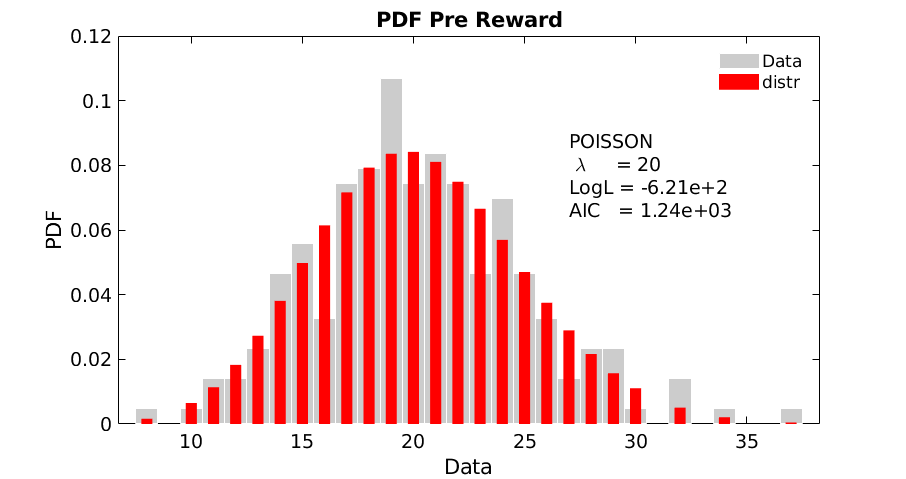
\includegraphics[scale=0.25]{figures/PreRewDistr_An1neu6_FSI.png}
    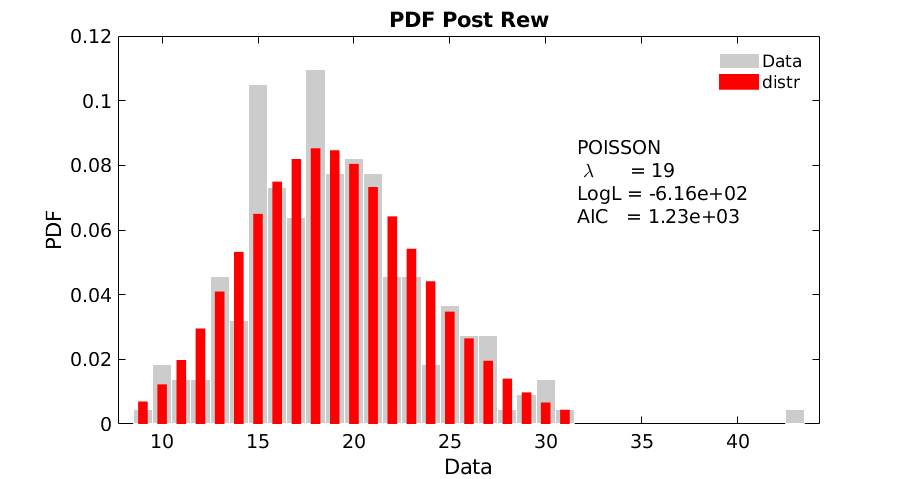
\includegraphics[scale=0.25]{figures/PostRewDistr_An1neu6_FSI_.png}
    \caption{Example of one unit firing rate distribution in the pre-reward range [-0.5 s,0s] and during the post reward period [0s,0.5s], choosing as starting time the reward delivery.}
    \label{fig:DistributionEx}\end{figure}
%%%%%%However, in some cases it makes sense to try to match the domain of the link function to the range of the distribution function's mean, or use a non-canonical link function for algorithmic purposes, for example Bayesian probit regression. 
\section{Regression}
\label{sec:Regression}
\section{Conclusion}
From the regression analysis, as one could predict, VS units emerged to be correlated with the $Q$ values, in particular FSI units show this correlation very clear.
{\color{red}insert percentage of units correlated and in which period, detailed with how many units are part of assemblies and add as well.}
\begin{figure}
    \centering
    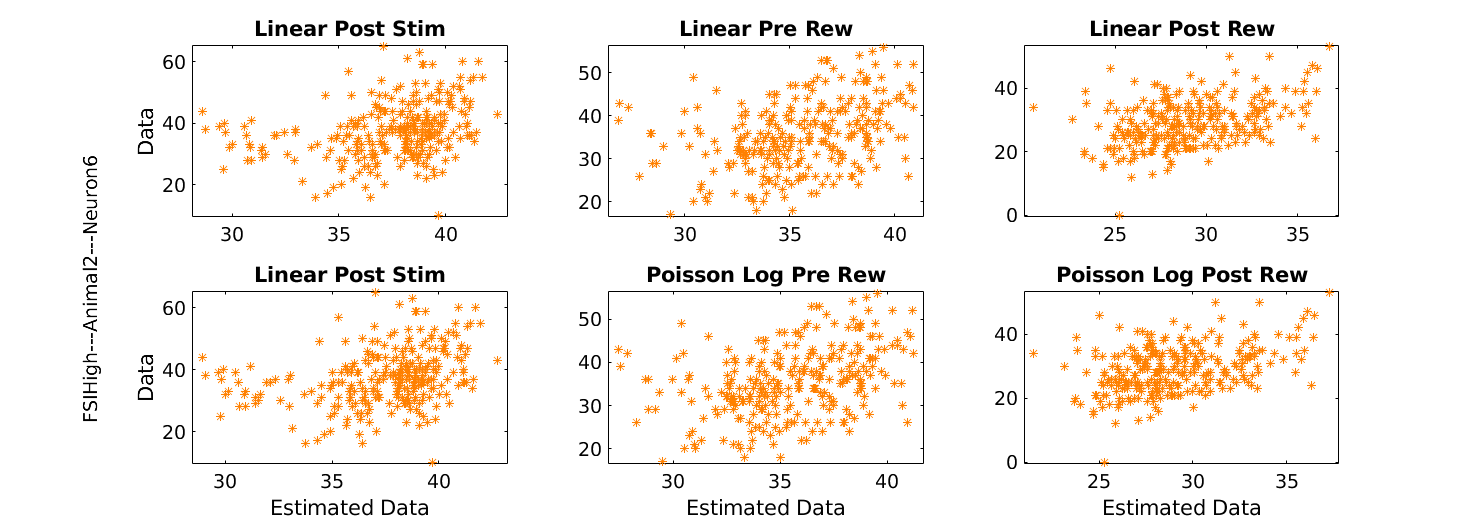
\includegraphics[scale=0.3]{figures/y_yhatAnimal2neu6_FSI.png}
    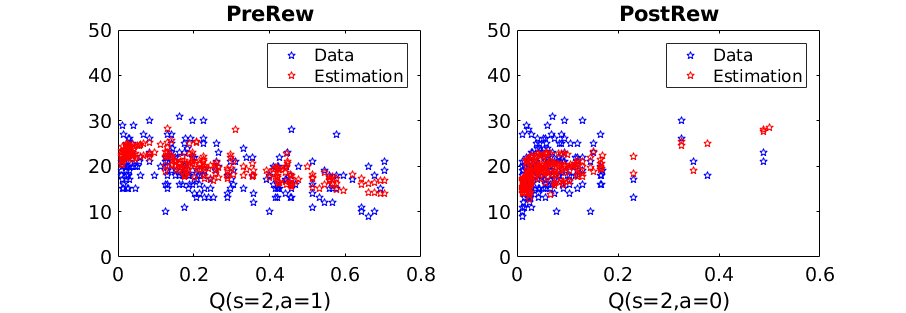
\includegraphics[scale=0.3]{figures/CorrelationExAn1neu6_RightAx.png}
    \caption{Caption}
    \label{fig:my_label}
\end{figure}